
%------------------------------------------------   
\section{Data Analysis}

El Análisis Exploratorio de Datos \textit{(Exploratory Data Analysis (EDA))} \citep{eda} es muy importante para poder obtener información y conocimiento acerca del dataset. Así pues, en esta sección se van a aplicar distintas técnicas para poder obtener qué productos químicos son los más frecuentes, qué cosméticos son los que presentan mayor número de productos químicos, cómo se distribuyen los datos en función de ciertos campos y cómo se distribuyen por cluster, la cantidad de productos químicos totales. Todo esto se encuentra implementado en el notebook \code{src/clustering-and-data-analysis.ipynb} \citep{master}.



%------------------------------------------------   
\subsection{Obtención de los productos químicos más frecuentes en los cosméticos}
\label{sec:casid-histograms}

La obtención de los productos químicos más frecuentes en los cosméticos se va a realizar realizando histogramas sobre el campo \code{CasId} del dataset. La Figura \ref{fig:histogram-casid-basic} muestra el histograma sobre todo el dataset, donde se puede observar que entre los valores 600 y 700 hay un gran volumen. \\

Concretamente, este volumen se encuentra entre los valores 656 and 658. La Figura \ref{fig:histogram-casid-656-658} muestra el histograma entre dichos valores, donde se puede observar que el volumen se encuentra en el producto químico con \code{CasId} 656, cuyo nombre es: 
\begin{itemize}
 \item \code{656 - Titanium dioxide}.
\end{itemize}

y pertenece al Cluster 0. 

\begin{figure}[!th]
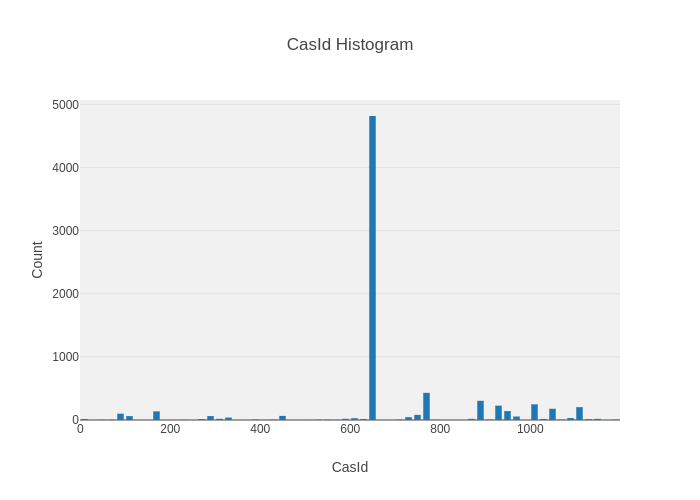
\includegraphics[scale=0.5]{figures/histogram-casid-basic}
\centering
\caption{Histograma sobre el campo \code{CasId}.}
\label{fig:histogram-casid-basic}
\end{figure}

\begin{figure}[!th]
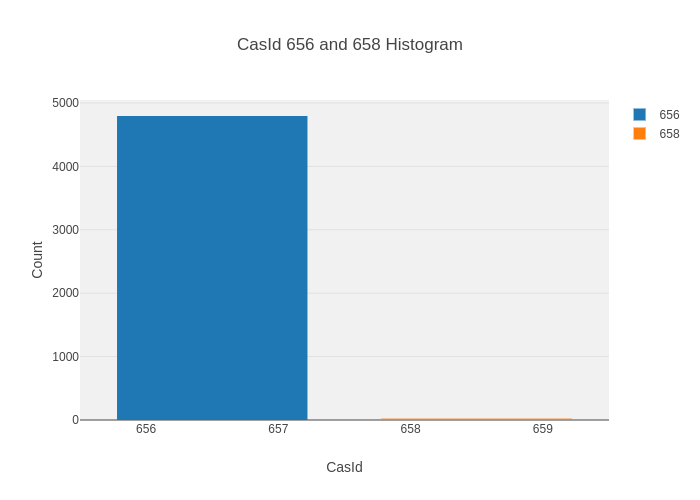
\includegraphics[scale=0.5]{figures/histogram-casid-656-658}
\centering
\caption{Histograma de los valores 656 y 658 del campo \code{CasId}.}
\label{fig:histogram-casid-656-658}
\end{figure}


Sin embargo, como podemos observar en la Figura \ref{fig:histogram-casid-basic}, la diferencia de volumen es muy grande entre el \code{CasId} 656 y el resto. Por lo que se va a realizar los mismos pasos anteriores, pero quitando el \code{CasId} 656 de los datos. \\

La Figura \ref{fig:histogram-casid-without656} muestra el histograma sobre el campo \code{CasId} del dataset sin el \code{CasId} 656 y, además, diferenciando por cluster, donde se puede observar que sigue habiendo un gran volumen entre los valores 700 y 800 y que pertenecen al Cluster 0.


\newpage
\begin{figure}[!th]
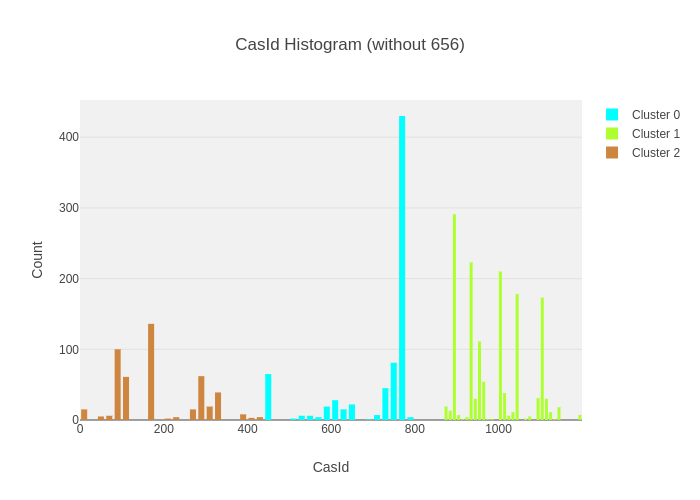
\includegraphics[scale=0.5]{figures/histogram-casid-without656}
\centering
\caption{Histograma sobre el campo \code{CasId} sin el \code{CasId} 656, diferenciando por cluster.}
\label{fig:histogram-casid-without656}
\end{figure}

Concretamente, este volumen se encuentra entre los valores 773 y 776. La Figura \ref{fig:histogram-casid-773-776} muestra el histograma de dichos valores, donde se puede apreciar que el \code{CasId} 773 tiene mayor volumen. El nombre de cada uno de los productos químicos es:

\begin{itemize}
 \item \code{773 - Retinol/retinyl esters, when in daily dosages in excess of 10,000 IU, or 3,000 retinol equivalents}.
 \item \code{776 - Silica, crystalline (airborne particles of respirable size)}.
\end{itemize}


\newpage
\begin{figure}[!th]
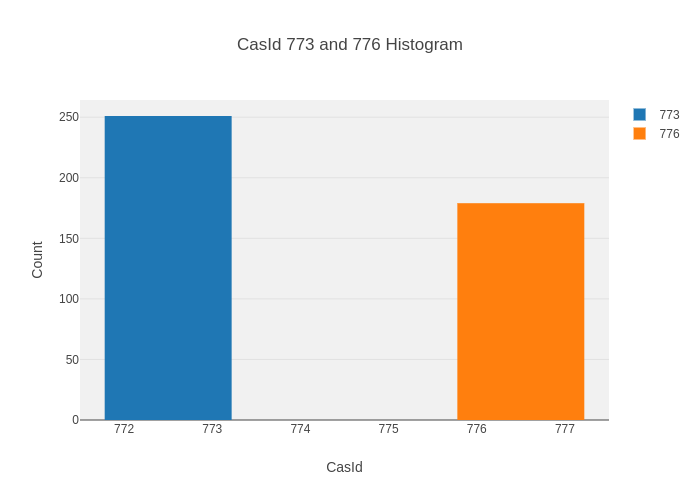
\includegraphics[scale=0.49]{figures/histogram-casid-773-776}
\centering
\caption{Histograma de los valores 773 y 776 del campo \code{CasId}.}
\label{fig:histogram-casid-773-776}
\end{figure}









%------------------------------------------------   
\subsection{Obtención de los cosméticos con mayor número de productos químicos}
\label{sec:subcategoryid-histograms}

Con la misma filosofía que en la sección \ref{sec:casid-histograms}, se van a realizar histogramas sobre el campo \code{SubCategoryId} para obtener los cosméticos que presentan mayor número de productos químicos. La Figura \ref{fig:histogram-subcategoryid-per-cluster} muestra el histograma sobre el campo \code{SubCategoryId} de todo el dataset diferenciando por cluster.

\begin{figure}[!th]
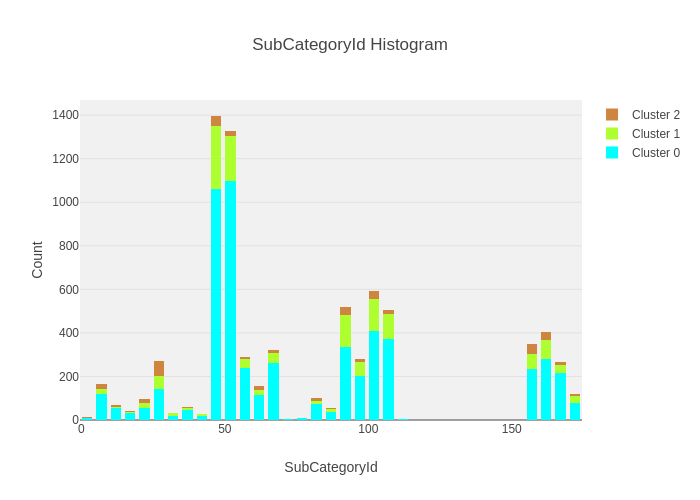
\includegraphics[scale=0.5]{figures/histogram-subcategoryid-per-cluster}
\centering
\caption{Histograma sobre el campo \code{SubCategoryId} diferenciando por cluster.}
\label{fig:histogram-subcategoryid-per-cluster}
\end{figure}


Como se puede observar, hay un gran volumen de registros que pertenecen al Cluster 0, esto es debido al volumen que presenta el \code{CasId} 656 en todo el dataset. Por lo tanto, para poder hacer un estudio más detallado, se va a eliminar el \code{CasId} 656. Así pues, la Figura \ref{fig:histogram-subcategoryid-per-cluster-without656} muestra el mismo histograma que en la Figura \ref{fig:histogram-subcategoryid-per-cluster} pero sin el \code{CasId} 656. 

\begin{figure}[!th]
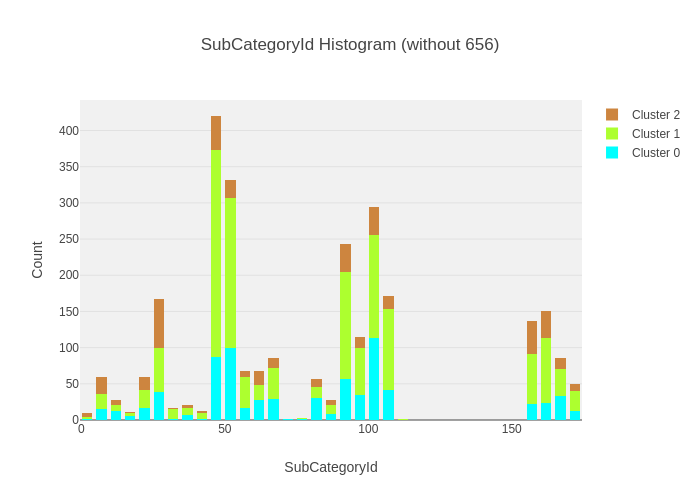
\includegraphics[scale=0.5]{figures/histogram-subcategoryid-per-cluster-without656}
\centering
\caption{Histograma sobre el campo \code{SubCategoryId} diferenciando por cluster, sin el \code{CasId} 656.}
\label{fig:histogram-subcategoryid-per-cluster-without656}
\end{figure}

Al igual que ocurrió con el campo \code{CasId}, se puede observar que entre los valores 40 y 50 del campo \code{SubCategoryId} se encuentra un volumen superior al resto. Concretamente, se encuentra entre los valores 45, 46, 48 y 49. La Figura \ref{fig:histogram-subcategoryid-45-49} muestra el histograma de dichos valores, donde se puede apreciar que el valor \code{SubCategoryId} 48 es el que tiene un volumen mayor. Además, también se puede observar que la gran mayoría de los registros pertenecen al Cluster 1. \\

El nombre de cada uno de los cosméticos es:

\begin{itemize}
 \item \code{45 - Blushes}.
 \item \code{46 - Eyeliner/Eyebrow Pencils}.
 \item \code{48 - Eye Shadow}.
 \item \code{49 - Face Powders}.
\end{itemize}


\newpage
\begin{figure}[!th]
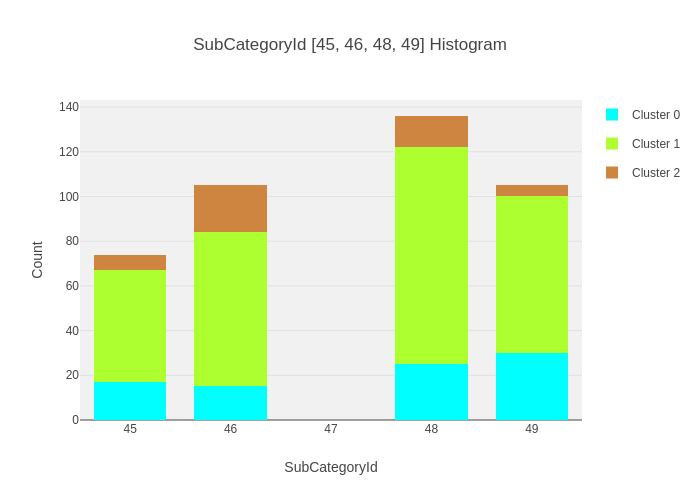
\includegraphics[scale=0.5]{figures/histogram-subcategoryid-45-49}
\centering
\caption{Histograma de los valores 45, 46, 48 y 49 del campo \code{SubCategoryId} diferenciando por cluster, sin el \code{CasId} 656.}
\label{fig:histogram-subcategoryid-45-49}
\end{figure}



\newpage
%------------------------------------------------   
\subsection{Distribución del dataset}
\label{sec:dataset-distribution}

En la Figura \ref{fig:splom-data-aggregated} se muestra la distribución del dataset en función de los campos \code{CasId}, \code{InitialDateReported\_Year}, \code{MostRecentDateReported\_Year} y \code{SubCategoryId}, diferenciando por cluster, en el que se puede observar que en los primeros años (2009 y 2010) fue cuando se reportaron la gran mayoría de los productos químicos y que en los años siguientes han ido reportándose de una manera muy equilibrada.

\begin{figure}[!th]
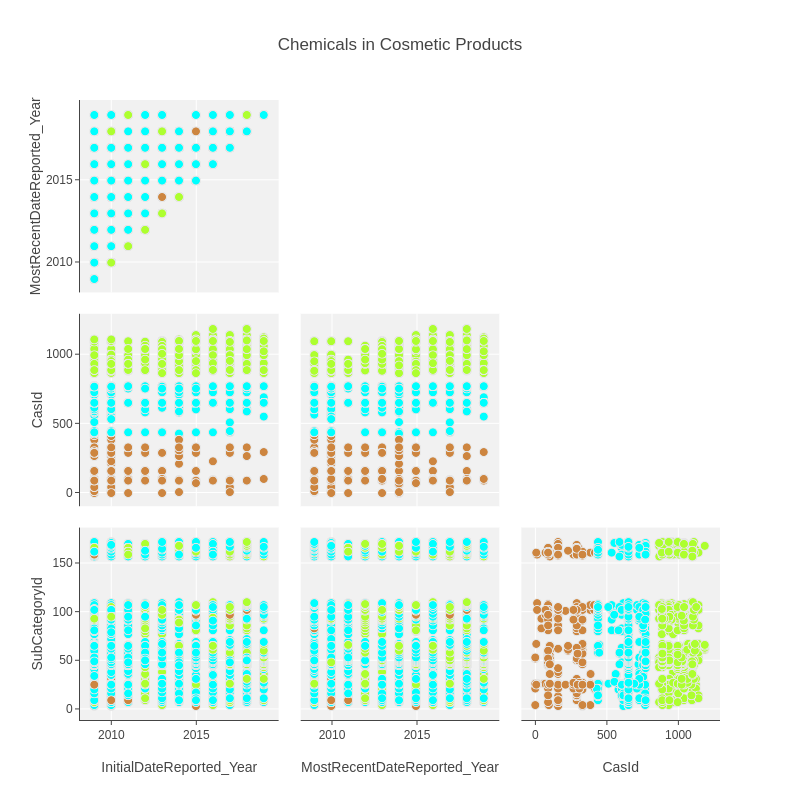
\includegraphics[scale=0.5]{figures/splom-data-aggregated}
\centering
\caption{Distribución del dataset en función de los campos \code{InitialDateReported\_Year}, \code{MostRecentDateReported\_Year}, \code{SubCategoryId} y \code{CasId}.}
\label{fig:splom-data-aggregated}
\end{figure}




\newpage
%------------------------------------------------   
\subsection{Distribución de la cantidad de productos químicos por cluster}
\label{sec:chemicals-per-cluster}

Hasta ahora se han estudiado la frecuencia en la que aparecen los productos químicos y los cosméticos en el dataset. En este punto, se va a estudiar la distribución de la cantidad de productos químicos en cada uno de los clusters, esto es: la suma del campo \code{ChemicalCount} distribuido en cada uno de los clusters. La Figura \ref{fig:pie-sum-chemicalcount} muestra esta distribución.


\begin{figure}[!th]
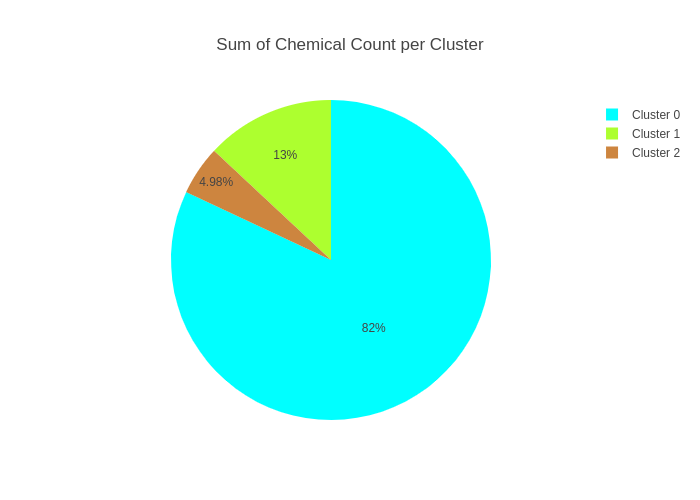
\includegraphics[scale=0.46]{figures/pie-sum-chemicalcount}
\centering
\caption{Distribución de la suma del campo \code{ChemicalCount} por cada cluster.}
\label{fig:pie-sum-chemicalcount}
\end{figure}

Al igual que pasaba en la sección \ref{sec:subcategoryid-histograms}, el alto porcentaje del Cluster 0 se debe al \code{CasId} 656. Por lo que, la Figura \ref{fig:pie-sum-chemicalcount-without656} muestra la misma distribución eliminando el \code{CasId} 656 del dataset. Donde se puede observar que más del 50\% de los productos químicos se encuentran en el Cluster 1.

\begin{figure}[!th]
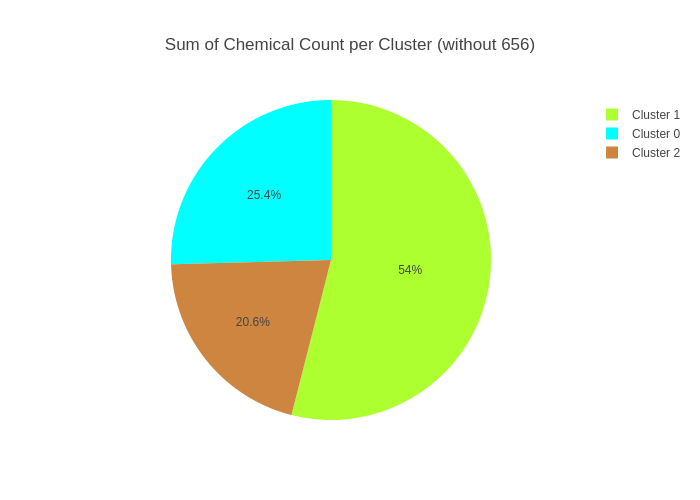
\includegraphics[scale=0.46]{figures/pie-sum-chemicalcount-without656}
\centering
\caption{Distribución de la suma del campo \code{ChemicalCount} por cada cluster, sin el \code{CasId} 656.}
\label{fig:pie-sum-chemicalcount-without656}
\end{figure}

















\newpage









